\section{CRSF-Protokoll}
CRSF ist ein Protokoll \cite{crsf_protokoll_spec} das für die Kommunikation von Radio Controlled (RC)
Geräten genutzt wird. Anders als wie bei z.B. S-Bus sind die Frame-Größen nicht
konstant, sondern werden auf Größe des Pakets angepasst. Das machte es zu einem
sehr flexiblen Protokoll, dass unter anderem die RC-Kanäle der Fernsteuerung, GPS
Daten und Übertragungsqualität übertragen kann, wie auch vieles weiteres.

\subsection{Aufbau eines Frames}
Der Anfang eines Frames ist immer gleich Aufgebaut. Es gibt einen Start Byte
(0xC8), Frame Länge und der Frame-Type. Danach folgt die Payload, die unterschiedlich lang
sein kann. Am Ende des Frames sitzt immer der CRC. Frames müssen mindestens 4
Byte lang sein und maximal 64 Byte.
\begin{figure}[h]
    \centering
    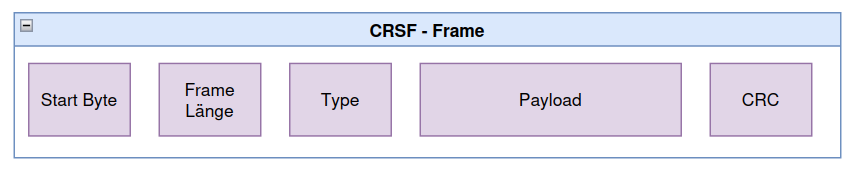
\includegraphics[width=\textwidth]{Bilder-Grafiken/Matthias/Fernsteuerung/CRSF-Frame.png}
    \caption{Aufbau des CRSF-Frames \cite{crsf_protokoll_spec}}
\end{figure}

\subsection{Protokoll Schnittstelle}
Das CRSF-Protokoll wird wie die meisten anderne RC-Fernsteuerungsprtokolle über
UART übertragen. In der CRSF-Specification \cite{crsf_protokoll_spec} werden
drei Arten der Schnittstellen beschrieben. \grqq Single-Wire Half-Duplex
UART\grqq, \grqq Dual-Wire Full-Duplex UART\grqq und \grqq Multi-master I2C
(BST)\grqq. Die Schnittstelle die der Radiomasterr XR1 Nano supported ist die
Full-Duplex UART schnittstelle.\\
Laut Specification ist diese defaultmäßig auf eine 416666 Baudrate, 8N1 (8 Daten
Bits, keine Parität, und in Stopp-Bit) eingestellt. Sie muss mit 3.0 - 3.3 Volt
betrieben werden. Das UART Signal ist nicht invertiert, anders wie bei anderen
RC-Protokollen (z.B. S-Bus).

